\documentclass{beamer}
\usepackage{graphicx} % Required for inserting images

\title{Two sample z/t test}
\author{}
\date{}

\begin{document}

\frame{\titlepage}

\begin{frame}[t]
\frametitle{Dataset: Setup}
\begin{itemize}
    \item We have used synthetic data for now, so we know the true shift.
    \item Reference sample $X \sim \mathcal{N}(0, I)$: each value is drawn from a bell curve with mean 0 and std 1.
    \item Each data point has $d = 10$ \textbf{features} (columns).
    \item Each sample has $n \in \{10, 20, 50, 100\}$ data points (rows).
    \item A new sample $Y$ is drawn with one thing changed.
    \item Each setting is repeated 100 times.
\end{itemize}
\vspace{0.3cm}
\centering
\begin{tabular}{c|cccc}
         & feature 1 & feature 2 & $\cdots$ & feature 10 \\ \hline
point 1  & 0.3  & -1.2 & $\cdots$ & 0.0 \\
$\vdots$ & $\vdots$ & $\vdots$ & & $\vdots$ \\
point $n$ & 0.5 & -0.3 & $\cdots$ & -0.8 \\
\end{tabular}
\end{frame}

\begin{frame}[t]
\frametitle{Dataset: Shifts}
\small

\centering
\begin{tabular}{@{}l p{0.73\textwidth}@{}}
\textbf{Shift} & \textbf{What changes in $Y$} \\
\hline
Mean & Each feature's mean shifts by $a/\sqrt{10}$. \\
Variance & Each feature's standard deviation is multiplied by $s$. \\
Heavy-tailed mean & Same mean shift, with Student-$t_3$ noise. \\
\end{tabular}

\vspace{0.3cm}

\begin{itemize}
    \setlength{\itemsep}{0.15cm}
    \setlength{\parskip}{0pt}

    \item \textbf{$a$ (mean shift):} Controls the shift magnitude.
    Levels: $a \in \{0, 0.4, 0.8, 1.2, 1.6\}$.

    \item \textbf{$s$ (scale shift):} Controls the spread.
    For example, $s=1.2$ increases the standard deviation by 20\%.

    \item \textbf{No shift:} $a=0$ and $s=1$; used to measure false alarms.

    \item \textbf{Heavy-tailed noise:} Produces more extreme values and tests robustness to violations of the noise assumptions.
\end{itemize}

\end{frame}

\begin{frame}[t]
\frametitle{Tests ($\alpha = 0.05$)}
\begin{itemize}
    \item \textbf{t-test}: compares the mean of each feature.
    \item \textbf{KS test}: compares the full distribution of eaution assumption).
    \item t-test and KS: report a shift if \textbf{any} of the 10 features has $p < 0.05$.
    \item \textbf{GLRT}: likelihood ratio under a Gaussian model.
    \item GLRT: reports a shift if $-2\log\Lambda$ is above the 95th percentile of $\chi^2_{20}$.
\end{itemize}
\end{frame}

\begin{frame}[t]
\frametitle{Introduction}
\begin{itemize}
    \item The two-sample z/t-test examines whether two populations have the same mean, using their observed samples.
    \vspace{0.5em}
    \item \textbf{$H_{0}$:  $\mu_{x} = \mu_{y}$}
    \item \textbf{$H_{1}:$  $\mu_{x} \ne \mu_{y}$}
    \vspace{0.5em}
    \item Two different distributions can have the same population mean.
    \vspace{0.5em}
    \begin{enumerate}
        \item \(X\sim\mathcal{N}(0,1)\) and \(Y\sim\mathcal{N}(0,4)\)
        \vspace{0.3em}
        \item \(X\sim\mathcal{N}(2,1)\) and \(Y\sim\operatorname{Exp}(\lambda=1/2)\)
    \end{enumerate}
    \vspace{0.5em}
    \item But, in some cases we might have some prior knowledge of the samples and know that both belong to the same distribution family (ex: Gaussian), and have the same population variance.
    \vspace{0.3em}
    \begin{itemize}
        \item In this case, if $\mu_{x} = \mu_{y}$, both distributions are same - what we want to check.
    \end{itemize}
\end{itemize}
    
\end{frame}

\begin{frame}[t]
\begin{itemize}
    \item Even if two populations have the same mean, two randomly drawn samples will generally have different sample means due to sampling variability.
    \vspace{0.3em}
    \item We want to determine whether the observed difference between the sample means is statistically significant enough to reject \(H_0\).
    
\end{itemize}
    
\end{frame}



\begin{frame}[t]
\frametitle{When is a mean difference significant?}
\begin{itemize}
    \item First we measure how much the sample means differ: $\bar{X}-\bar{Y}$
    \vspace{0.3em}
    \item Let's say we get D = 5. 
    \vspace{0.1em}
    \begin{enumerate}
        \item \textit{Situation A}: Values usually between 49 \& 51, so D = 5 is relatively large.
        \vspace{0.2em}
        \item \textit{Situation B}: Values usually between 0 \& 100, so D = 5 may be relatively small.
    \end{enumerate}
    \vspace{0.3em}
    \item The observed difference alone is insufficient. We must account for the natural variability of the sample means.
    \vspace{0.3em}
    \item We quantify this variability using the \textbf{standard error.}

\end{itemize}
    
\end{frame}

\begin{frame}[t]
\frametitle{Standard Error}
\begin{itemize}
    \item \textbf{Standard deviation} measures how spread out individual observations are around their mean.
    \item However, we are comparing sample means, not individual observations.
    \item Even if the population means are equal, the sample means can differ due to random sampling.
    \item Standard error (SE) measures how much a sample statistic (such as the sample mean) would vary across repeated random samples.
 \[
\boxed{
SE(\bar X-\bar Y)=
\sqrt{\frac{s_X^2}{n_X}+\frac{s_Y^2}{n_Y}}
}
\]
\end{itemize}
    
\end{frame}

\begin{frame}[t]
\frametitle{Test Statistic}
\[
\boxed{
t=\frac{\bar X-\bar Y}{SE(\bar X-\bar Y)}
}
\]

\begin{itemize}
    \item The further away this value is from 0, the more likely it is that we can reject $H_{0}$
    \vspace{0.3em}
    \item But how do we determine whether the observed t-value is sufficiently extreme to reject \(H_0\)? We calculate its \textbf{p-value.}
    \vspace{0.3em}
    \item Assuming \(H_0\) is true, the p-value is the probability of observing a test statistic at least as extreme as the one obtained.
    \vspace{0.3em}
    \item We compare the p-value against a chosen significance level, \(\alpha\) (typically 0.05).
    \vspace{0.3em} \[
\boxed{
\begin{aligned}
p<\alpha &\implies \text{Reject }H_0\\
p\geq\alpha &\implies \text{Fail to reject }H_0
\end{aligned}
}
\]
\end{itemize}
    
\end{frame}


\begin{frame}[t]
\frametitle{Z-test}
\begin{itemize}
    \item The difference between z-test and t-test is that in z-test, the population variances are known.
\end{itemize}
\vspace{0.5em}
\[
\boxed{z=\frac{\bar X-\bar Y}{\sqrt{\frac{\sigma_X^2}{n_X}+\frac{\sigma_Y^2}{n_Y}}}}
\]
\end{frame}


% ====================================================================
% NEW SECTION: KS test (added; all other frames are unchanged)
% Requires the figure file ks_gap.png next to this .tex file.
% ====================================================================

\begin{frame}[t]
\frametitle{KS Test: Introduction}
\begin{itemize}
    \item The Kolmogorov--Smirnov (KS) test examines whether two populations have the same \textbf{distribution}, not just the same mean, using their observed samples.
    \vspace{0.5em}
    \item \textbf{$H_{0}$:  $F_{X} = F_{Y}$}
    \item \textbf{$H_{1}:$  $F_{X} \ne F_{Y}$}
    \vspace{0.5em}
    \item Here $F$ is the cumulative distribution function (CDF): $F(x)$ is the probability that a value is at most $x$.
    \vspace{0.5em}
    \item The t-test cannot separate \(X\sim\mathcal{N}(0,1)\) from \(Y\sim\mathcal{N}(0,4)\), since both have mean 0. The KS test can, because their distributions differ.
    \vspace{0.5em}
    \item The KS test is \textbf{nonparametric}: it does not assume that the data are Gaussian or that the variances are equal.
\end{itemize}
\end{frame}

\begin{frame}[t]
\frametitle{Empirical CDF}
\begin{itemize}
    \item We do not know the true CDF, so we estimate it from a sample by counting.
    \item The \textbf{empirical CDF} is the fraction of the sample that is at most $x$:
 \[
\boxed{
\hat F_X(x)=\frac{1}{n_X}\sum_{i=1}^{n_X}\mathbf{1}\{X_i\le x\}
}
\]
    \item Here $\mathbf{1}\{\cdot\}$ is 1 when the condition is true and 0 otherwise.
    \vspace{0.3em}
    \item Example: for $X=\{1,2,4,7\}$, $\hat F_X(3)=\frac{2}{4}=0.5$.
    \vspace{0.3em}
    \item It is a staircase: it starts at 0, rises by $1/n_X$ at each data point, and ends at 1.
    \item Even if $H_0$ is true, $\hat F_X$ and $\hat F_Y$ will differ slightly due to sampling variability.
\end{itemize}
\end{frame}

\begin{frame}[t]
\frametitle{KS Statistic}
\small
\[
\boxed{
D=\max_{x}\left|\hat F_X(x)-\hat F_Y(x)\right|
}
\]

\begin{itemize}
    \item $D$ is the largest vertical gap between the two empirical CDFs, so $0 \le D \le 1$.
    \item The further $D$ is from 0, the more likely it is that we can reject $H_{0}$.
    \item Both CDFs only change at data points, so it is enough to check the gap at the data points.
\end{itemize}

\centering
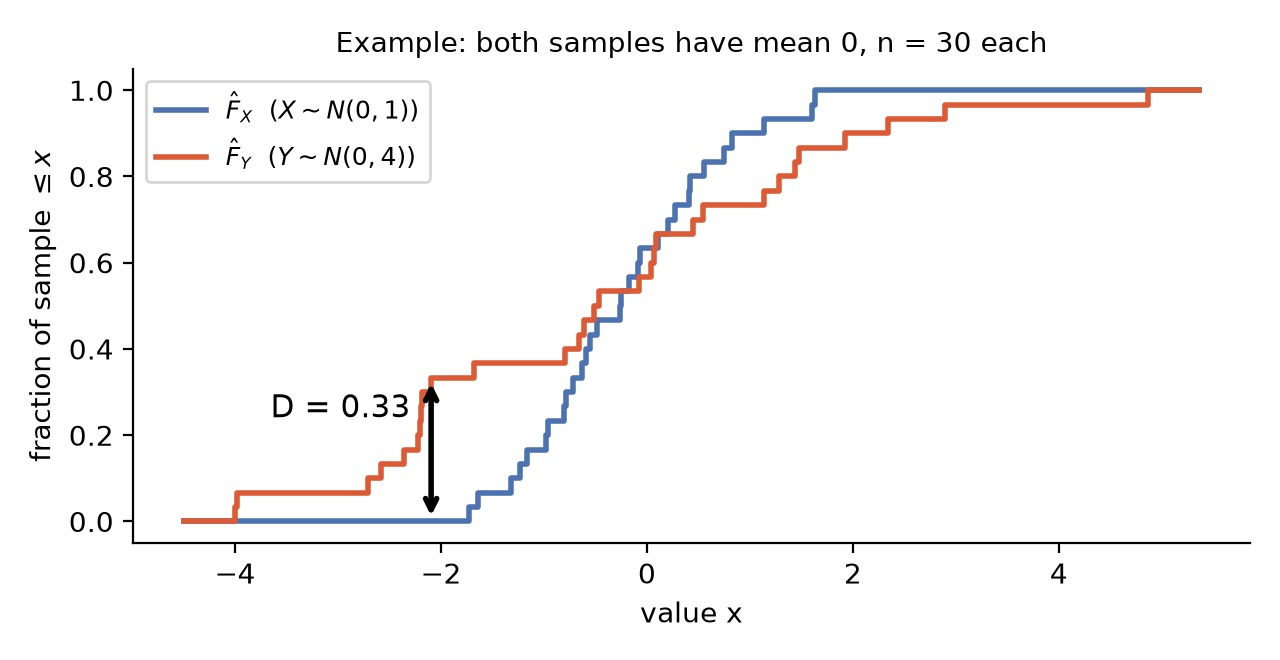
\includegraphics[width=0.62\textwidth]{ks_gap.png}
\end{frame}

\begin{frame}[t]
\frametitle{KS Test: p-value and Decision}
\begin{itemize}
    \item How large must $D$ be? We compare it with how large it would typically be if $H_0$ were true, just as the t-test compares the difference of means with the standard error.
    \vspace{0.3em}
    \item For continuous data, the distribution of $D$ under $H_0$ is the same whatever the data distribution is, so no Gaussian assumption is needed.
    \vspace{0.3em}
    \item For large samples, we reject $H_0$ at $\alpha = 0.05$ if
 \[
\boxed{
\sqrt{\frac{n_X n_Y}{n_X+n_Y}}\;D > 1.358
}
\]
    \item The factor $\sqrt{n_X n_Y/(n_X+n_Y)}$ rescales $D$ for the sample sizes, similar to dividing by the standard error in the t-test.
    \vspace{0.3em}
    \item For small samples the exact distribution of $D$ is used. The p-value is the probability, assuming $H_0$ is true, of observing a $D$ at least as large as the one obtained, and the decision rule is the same: reject $H_0$ if $p<\alpha$.
\end{itemize}
\end{frame}

\begin{frame}[t]
\frametitle{What the KS Test Can See}
\begin{itemize}
    \item The KS test reacts to \textbf{any} change in the distribution: a shift in the mean, a change in the variance, or a change in shape.
    \vspace{0.3em}
    \item The t-test reacts only to a change in the mean. If the mean is unchanged, it cannot see a variance shift.
    \vspace{0.3em}
    \item The price of this generality: for a pure mean shift in Gaussian data, the t-test is the more powerful test, since it uses exactly the information that matters.
    \vspace{0.3em}
    \item In our experiment, the KS test is applied to each of the 10 features separately, and we report a shift if \textbf{any} feature has $p<0.05$ (the same rule as the t-test).
\end{itemize}

\vspace{0.2em}
\centering
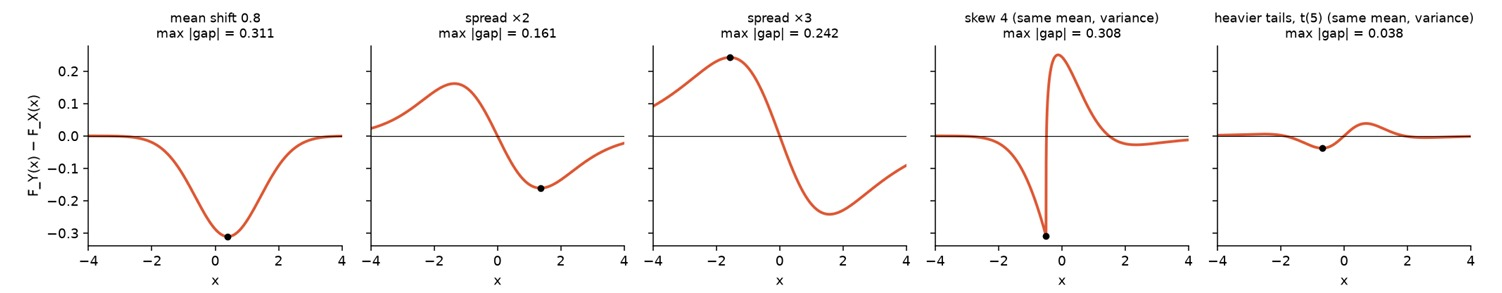
\includegraphics[width=\textwidth]{ks_gaps.png}
\end{frame}

% ====================================================================
% END OF NEW SECTION
% ====================================================================


\begin{frame}[t]
\frametitle{Results: False Alarms (no shift)}
\centering
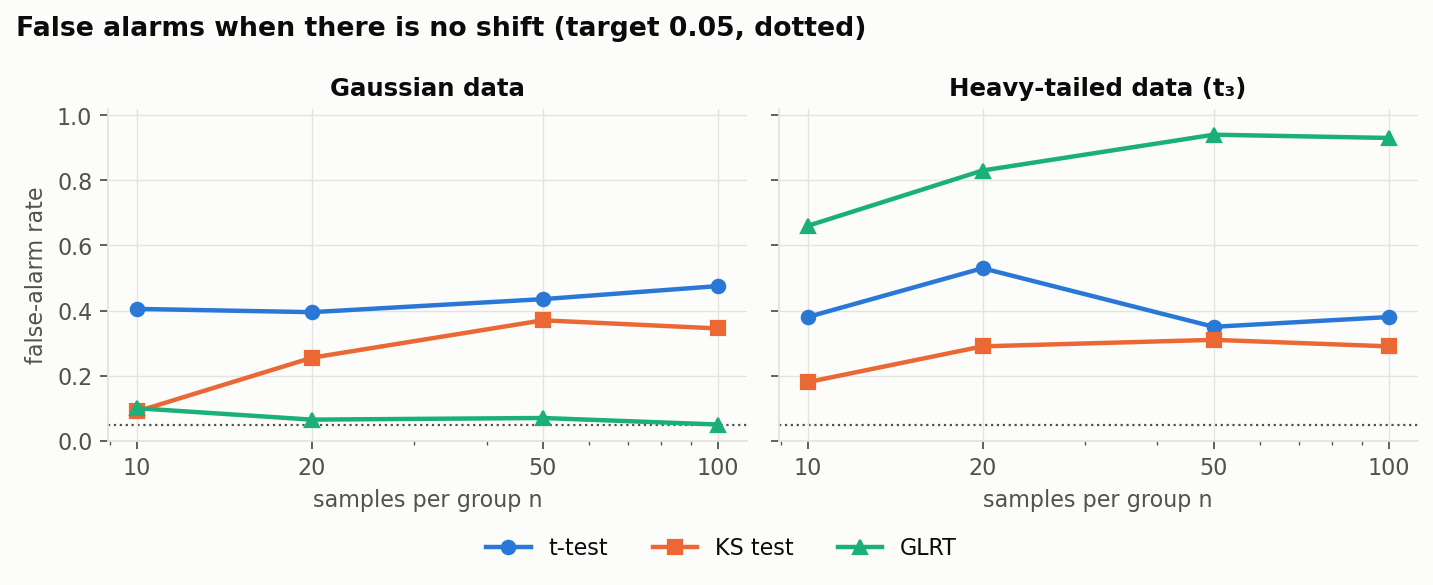
\includegraphics[width=\textwidth]{01_false_alarms.png}
\begin{itemize}
    \item t-test and KS: 30--50\% false alarms, because 10 features at 5\% each give $1 - 0.95^{10} \approx 40\%$.
    \item GLRT on Gaussian data: about 5\%, as it should be.
    \item GLRT on heavy-tailed data: up to 93\% false alarms.
\end{itemize}
\end{frame}

\begin{frame}[t]
\frametitle{Results: Detection Rate ($n = 100$)}
\centering
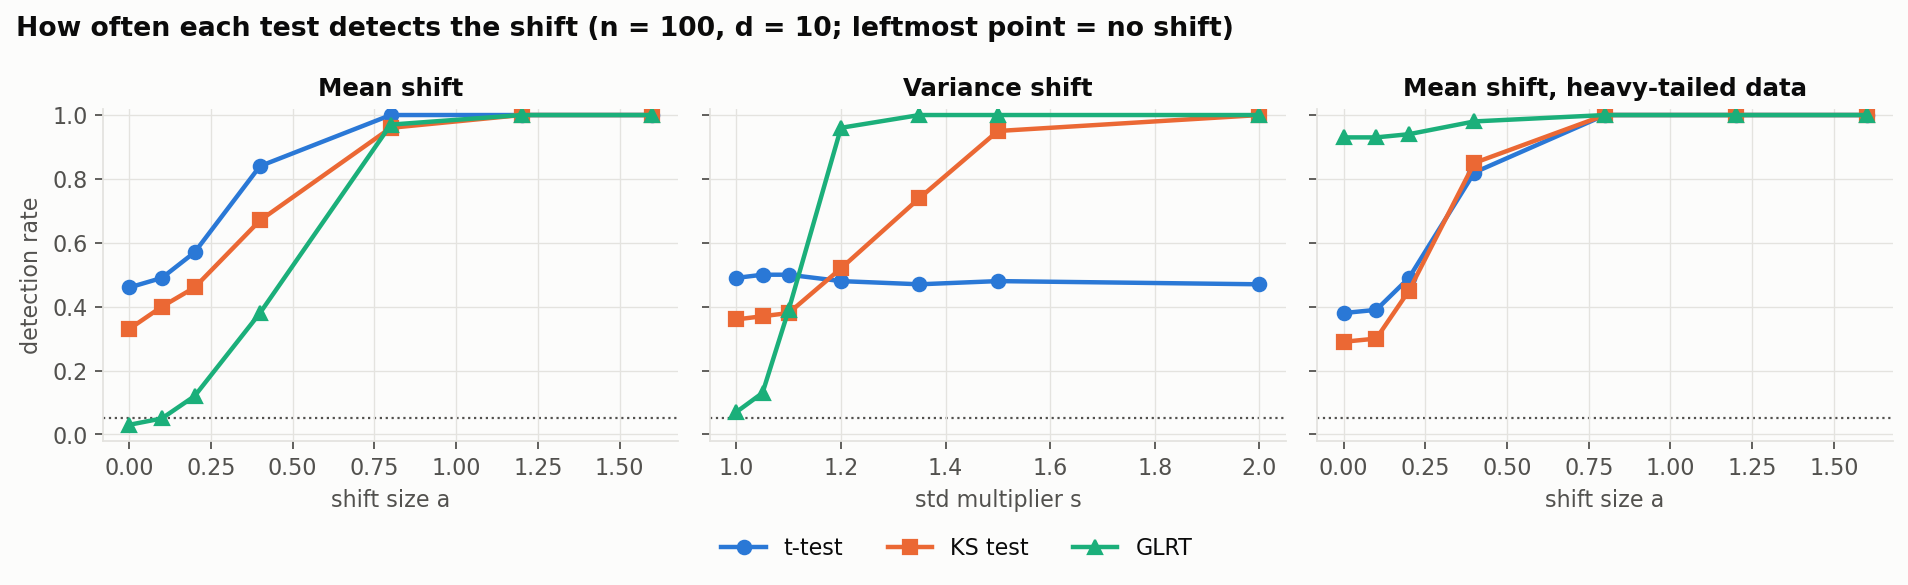
\includegraphics[width=\textwidth]{02_detection.png}
\begin{itemize}
    \item \textbf{Mean}: all three tests reach about 100\% by $a = 0.8$.
    \item \textbf{Variance}: the t-test cannot see it; GLRT is best (96\% vs 52\% for KS at $s = 1.2$).
    \item \textbf{Heavy-tailed}: GLRT reports a shift even with no shift (93\%), so its detections are meaningless.
\end{itemize}
\end{frame}

\begin{frame}[t]
\frametitle{Results: Does the GLRT Follow $\chi^2_{20}$?}
\centering
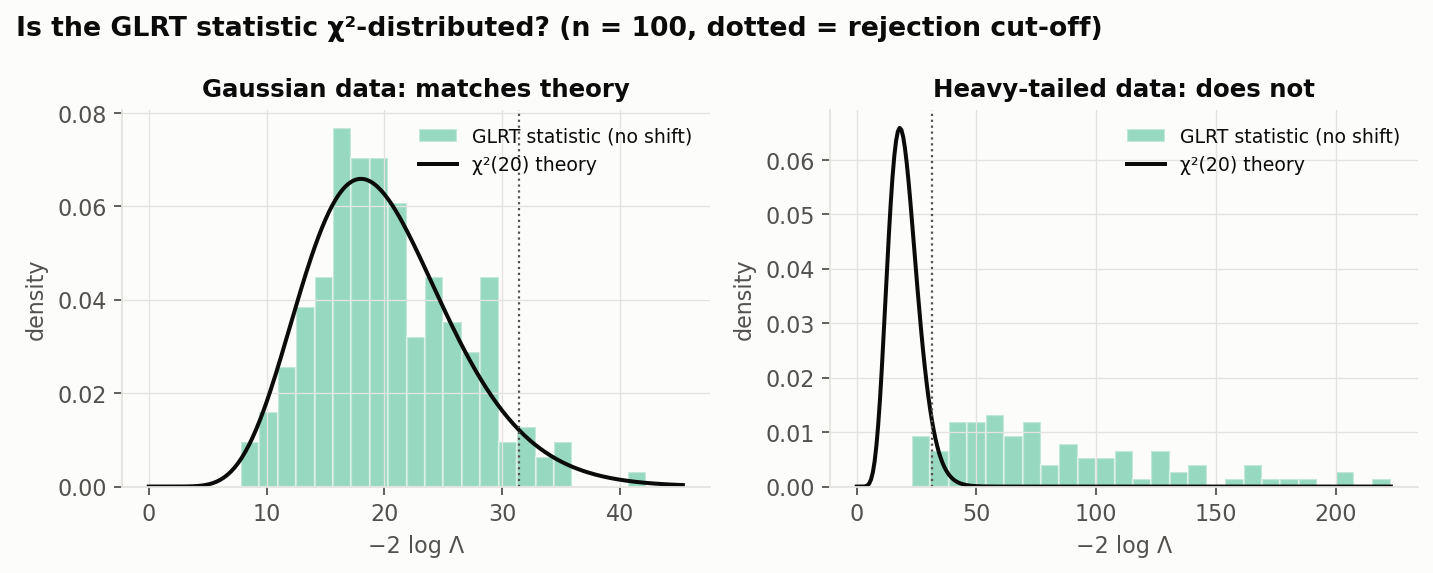
\includegraphics[width=0.85\textwidth]{03_glrt_vs_chi2.png}
\begin{itemize}
    \item Gaussian data: matches $\chi^2_{20}$, so its p-values
    \item Heavy-tailed data: values are far above $\chi^2_{20}$, so ordinary noise looks like a shift.
\end{itemize}
\end{frame}

\begin{frame}[t]
\frametitle{Results: Summary ($n = 100$)}
\small
\centering

\begin{tabular}{l|cccc}
 & \textbf{No shift} & \textbf{Mean} & \textbf{Variance} & \textbf{Heavy-tailed} \\
 & \textbf{(false alarm)} & $a = 0.8$ & $s = 1.2$ & \textbf{(no shift)} \\
\hline
t-test & 0.48 & 1.00 & 0.48 & 0.38 \\
KS     & 0.35 & 0.96 & 0.52 & 0.29 \\
GLRT   & \textbf{0.05} & 0.97 & \textbf{0.96} & 0.93 \\
\end{tabular}

\vspace{0.4cm}

\begin{itemize}
    \item GLRT is the best test when the data is Gaussian, but fails when the Gaussian assumption is violated.
    \item Testing each feature separately without a multiple-testing correction inflates the false alarm rate.
    \item The GLRT requires a suitable distributional model for its reference distribution to be valid.
\end{itemize}
\end{frame}

\end{document}